\chapter{Policy Evaluation}\label{C:us}

This section outlines my evaluation strategies, tests performed, and presents and discusses the results of evaluation conducted on the developed web scrapers. It then presents an evaluation of the policies and hypotheses formulated during analysis of data gathered. 

%Performance

%Resistance to Detection

%Logging



\section{Policy Evaluation}

This section outlines my evaluation strategies, tests performed, and presents and discusses the results of evaluation conduceted on the developed system. 

In order to evaluate my solution I need to refer back to the requirements gathered at the beginning of the project. 

- These requirements will be moved to the Requirements Analysis section... is just useful to have them stored here for easy referrals. 

\begin{itemize}
\item Develop a set of Policies that can be used to ...
\item Develop a metric of reliability of information gathered, based on privacy settings.
\item Potential to Develop an Interface with Filip Dimitrievski's project. Re-using my web-scraping libraries could be useful for his project. (Probably not going to happen)
\item Aggregate data for storage into GRAft
\end{itemize}

Non-Functional Requirements:
\begin{itemize}
\item Privacy Protection
\item Maintainability and Resistance to User-Interface Changes
\item Performance of Scrapers
\item Ability to Resist Blocking Detection, and Recover from Failure
\end{itemize}

\section{Policies}

\subsection{Correlation of Impact Factor vs Bucketed Impacts}

\begin{figure}[h!]
\centering
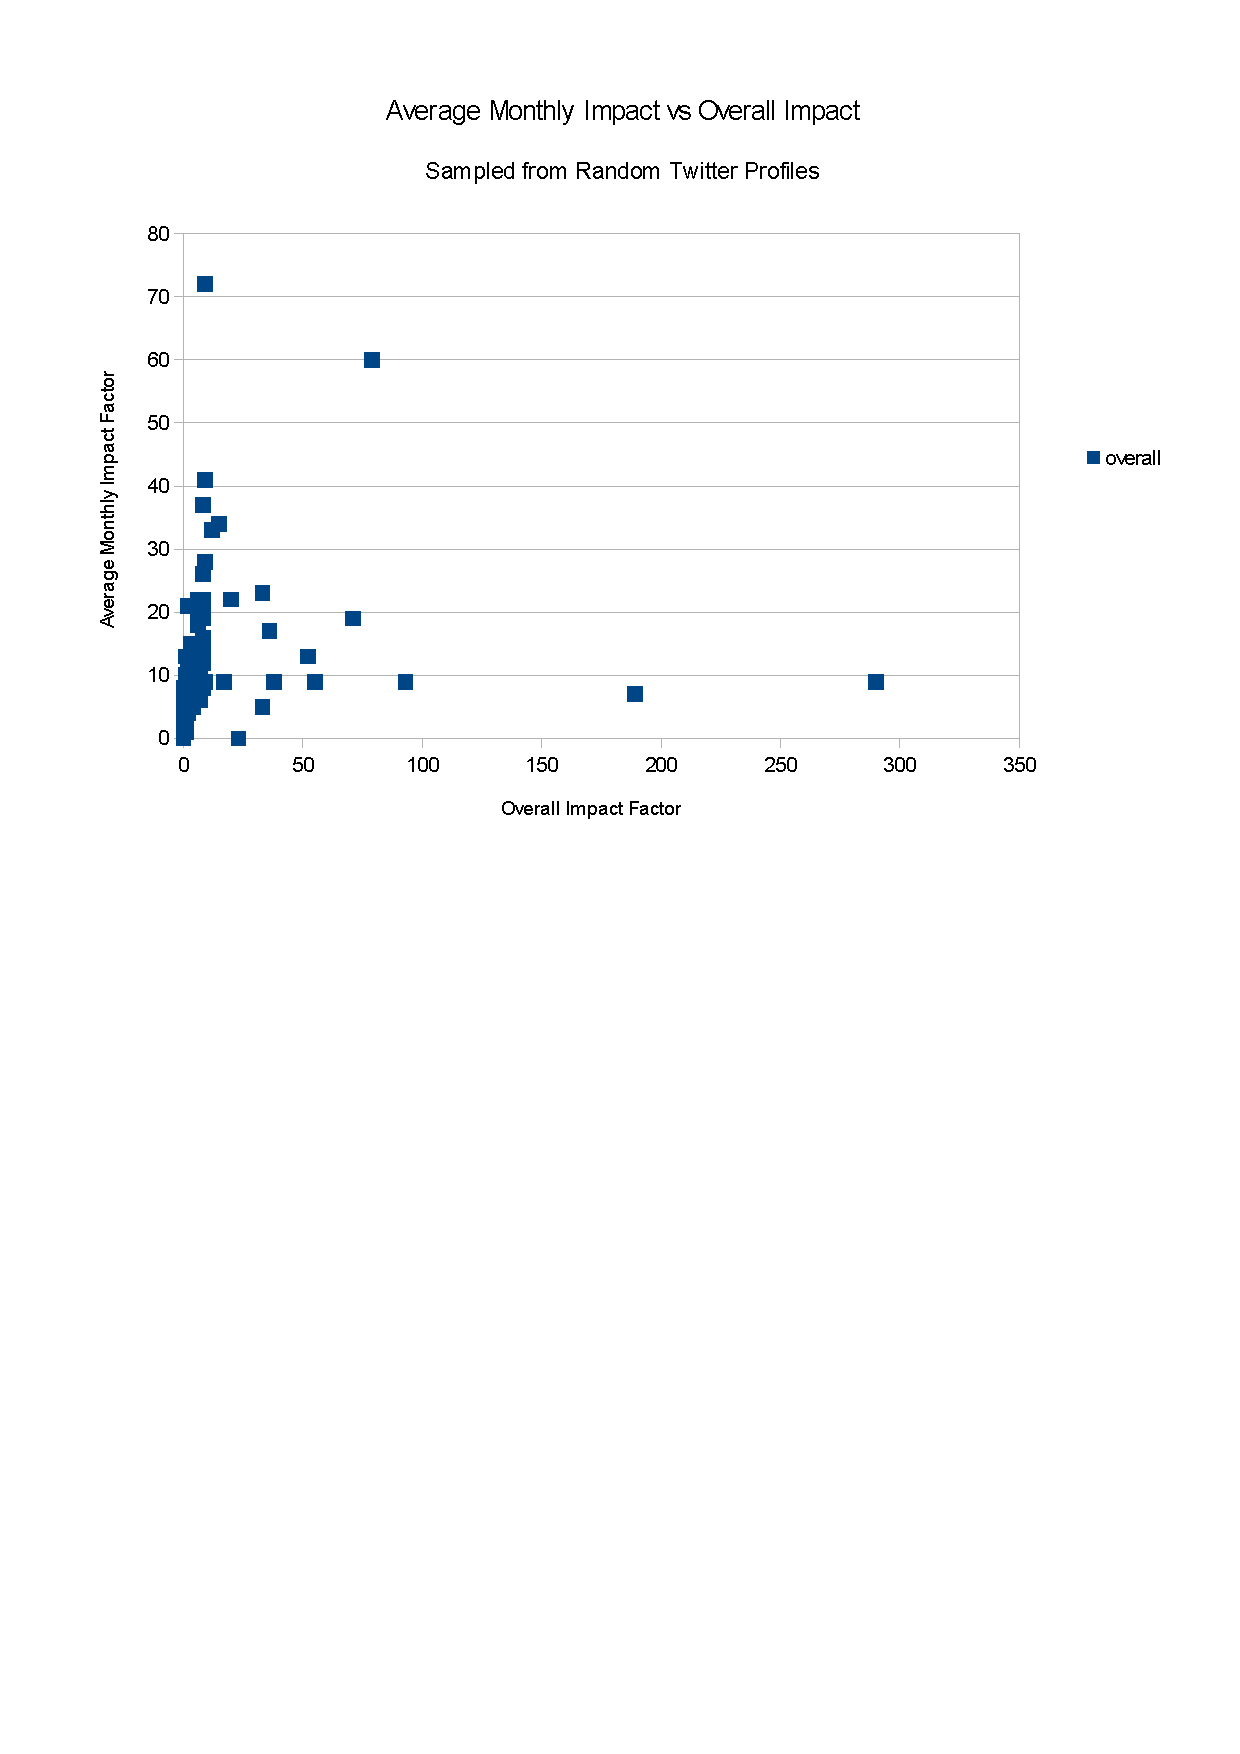
\includegraphics[width=400px]{Images/monthly_impact_vs_overallv2.pdf}
\caption{Monthly Impact against Overall Impact}
\end{figure}

\begin{figure}[h!]
\centering
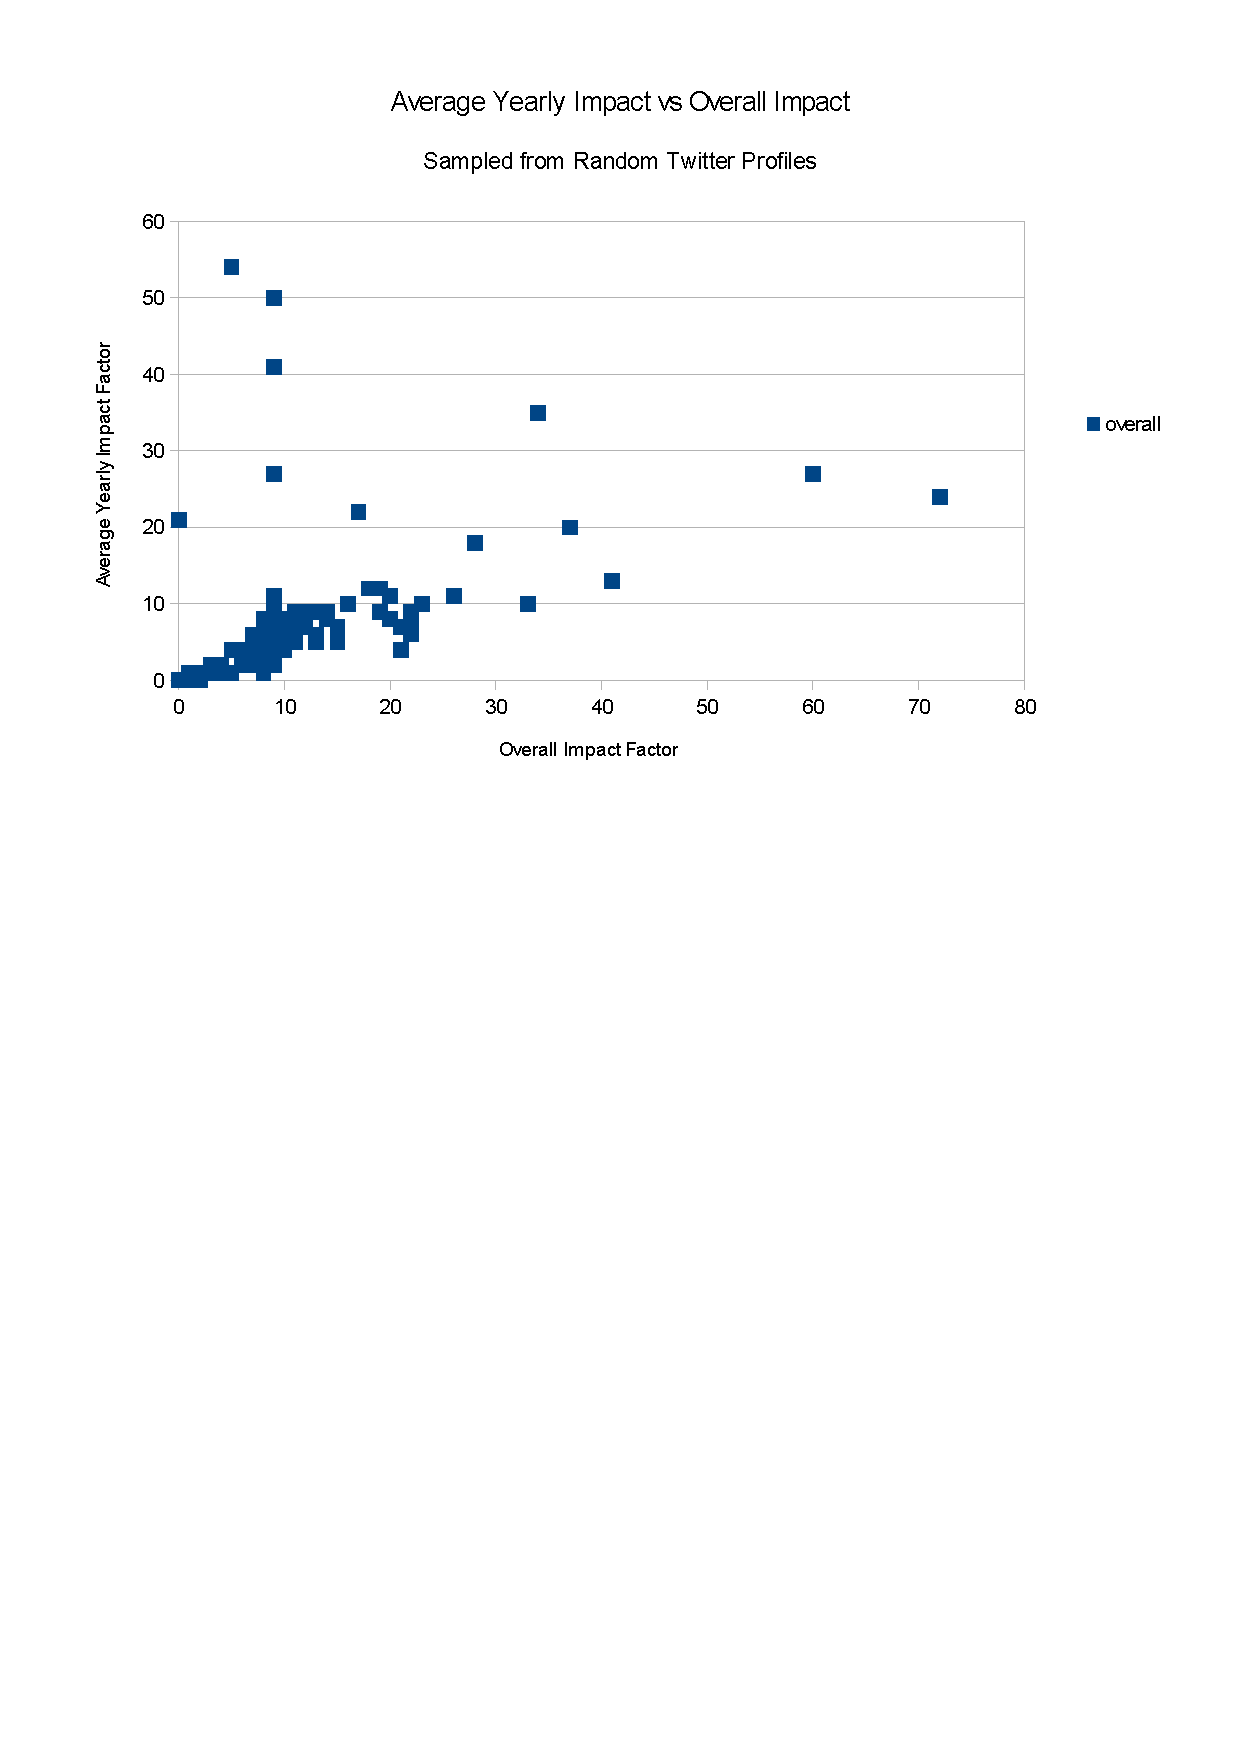
\includegraphics[width=400px]{Images/yearly_impact_vs_overallv2.pdf}
\caption{Yearly Impact against Overall Impact}
\end{figure}

One strategy for inferring reputation information that I looked at was through temporal bucketing of impact factor, into days, months, and years. The figures below show the relationship between people's mean monthly calculated impact factor (i.e. by calculating a person's impact score for each month, and then averaging these values over the total number of months), and the individual's overall impact score. I infer that there is a weak relationship between average monthly impact and overall impact (Pearson's correlation coefficient of 0.273(3 s.f.)), and a stronger relationship between average yearly impact and overall impact (r=0.689(3 s.f.))\\

\noindent What I believe this data shows is that the impact factor is favourable to individuals who are consistent on Twitter over time. 

\subsection{Results of Monthly Bucketing}

By applying the impact factor formula to individuals on a monthly basis, we are able to generate an impression of how regularly active a person is. The data also reveals how influential the person has been per month. This assists when comparing individuals who are consistently strongly influential (e.g. Barack Obama, companies such as instagram), with those who are popular for a limited period only. I looked at comparing different bucket sizes for this temporal aggregation. Days, months, and years were used as buckets, with monthly aggregation clearly showing the strongest and more interesting trends. 

\begin{figure}[h!]
\centering
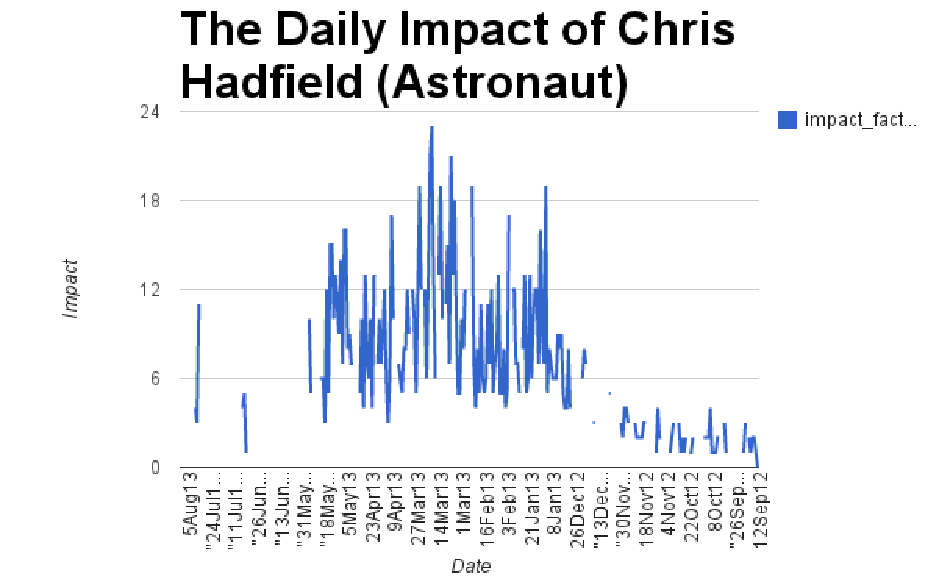
\includegraphics{Images/daily_impact_chris_hadfield.pdf}
\caption{The Daily Impact of Chris Hadfield - Famous Astronaut}
\end{figure}

\begin{figure}[h!]
\centering
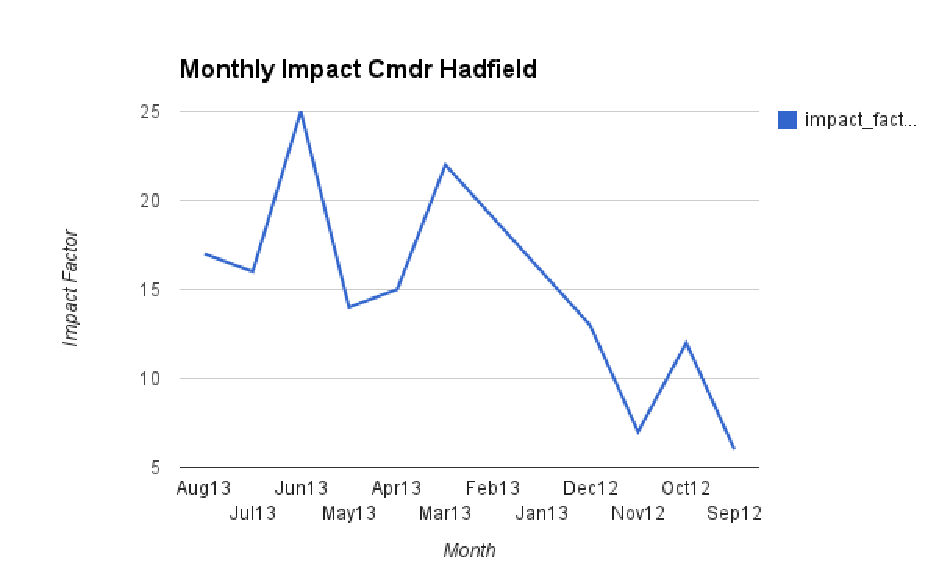
\includegraphics{Images/monthly_impact_chris_hadfield.pdf}
\caption{The Monthly Impact of Chris Hadfield - Famous Astronaut}
\end{figure}

\begin{figure}[h!]
\centering
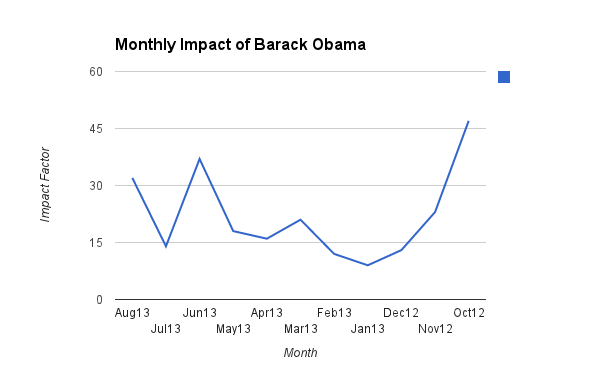
\includegraphics{Images/monthly_impact_barack_obama.png}
\caption{The Monthly Impact of Barack Obama - President of USA (As if you didn't know that)}
\end{figure}

We can see that the daily and monthly impact trends follow roughly the same curve, which should be expected. The difference is due to the strictness of the impact factor formula in classifying someone as 'influential'. It is very difficult to get a value much above 1 on a daily basis, unless you are very frequently both making use of the social media, and having people respond to this activity. 

\section{Scraper}

\subsection{Functional Requirements}

Aggregate data for storage into Graft - given that I am currently only storing data from Twitter this requirement has not yet been met.

Develop a metric of reliability of information gathered, based on privacy settings. Currently on Twitter there are two degrees of privacy - Open and Closed! Closed profiles means I cannot get any meaningful information, whereas on Open profiles I can get anything I want! Most profiles are open so this is not a concern. Profiles of celebrities etc are always set to open.

Developing a set of Policies - still in the production line, still experimenting with different ways of using the data.